%%%%%%%%%%%%%%%%%%%%%%%%%%%%%%%%%%%%%%%%%%%%%%%%%%%
%% LaTeX book template                           %%
%% Author:  Amber Jain (http://amberj.devio.us/) %%
%% License: ISC license                          %%
%%%%%%%%%%%%%%%%%%%%%%%%%%%%%%%%%%%%%%%%%%%%%%%%%%%

\documentclass[a4paper,11pt,oneside]{book}
\usepackage{modulestyle}

%%%%%%%%%%%%%%%%%%%%%%%%%%%%%%%%%%%%%%%%%%%%%%%%%%%%%%%%%
% Source: http://en.wikibooks.org/wiki/LaTeX/Hyperlinks %
%%%%%%%%%%%%%%%%%%%%%%%%%%%%%%%%%%%%%%%%%%%%%%%%%%%%%%%%%

%%%%%%%%%%%%%%%%%%%%%%%%%%%%%%%%%%%%%%%%%%%%%%%%%%%%%%%%%%%%%%%%%%%%%%%%%%%%%%%%
% 'dedication' environment: To add a dedication paragraph at the start of book %
% Source: http://www.tug.org/pipermail/texhax/2010-June/015184.html            %
%%%%%%%%%%%%%%%%%%%%%%%%%%%%%%%%%%%%%%%%%%%%%%%%%%%%%%%%%%%%%%%%%%%%%%%%%%%%%%%%
\newenvironment{dedication}
{
   \cleardoublepage
   \thispagestyle{empty}
   \vspace*{\stretch{1}}
   \hfill\begin{minipage}[t]{0.66\textwidth}
   \raggedright
}
{
   \end{minipage}
   \vspace*{\stretch{3}}
   \clearpage
}

%%%%%%%%%%%%%%%%%%%%%%%%%%%%%%%%%%%%%%%%%%%%%%%%
% Chapter quote at the start of chapter        %
% Source: http://tex.stackexchange.com/a/53380 %
%%%%%%%%%%%%%%%%%%%%%%%%%%%%%%%%%%%%%%%%%%%%%%%%
\makeatletter
\renewcommand{\@chapapp}{}% Not necessary...
\newenvironment{chapquote}[2][2em]
  {\setlength{\@tempdima}{#1}%
   \def\chapquote@author{#2}%
   \parshape 1 \@tempdima \dimexpr\textwidth-2\@tempdima\relax%
   \itshape}
  {\par\normalfont\hfill--\ \chapquote@author\hspace*{\@tempdima}\par\bigskip}
\makeatother

%%%%%%%%%%%%%%%%%%%%%%%%%%%%%%%%%%%%%%%%%%%%%%%%%%%
% First page of book which contains 'stuff' like: %
%  - Book title, subtitle                         %
%  - Book author name                             %
%%%%%%%%%%%%%%%%%%%%%%%%%%%%%%%%%%%%%%%%%%%%%%%%%%%

\newcommand{\BookTitle}{Data Structures and Algorithms}
\newcommand{\BookTitleFootnote}{A course in the Bachelor of Science in Computer
Science}

\newcommand{\BookSubtitle}{A Study Guide for Students of Sorsogon State University - Bulan Campus}
\newcommand{\BookSubtitleFootnote}{This book is a study guide for students of
Sorsogon State University - Bulan Campus taking up the course Data Structures
and Algorithms.}

\newcommand{\BookAuthorFirstName}{Jarrian Vince}
\newcommand{\BookAuthorLastName}{Gojar}
\newcommand{\BookAuthorName}{Jarrian Vince G. Gojar}
\newcommand{\BookAuthorURL}{https://github.com/godkingjay}

% Book's title and subtitle
\title{\Huge \textbf{\BookTitle}  \footnote{\BookTitleFootnote} \\
\huge \BookSubtitle \footnote{\BookSubtitleFootnote}}

% Author
\author{\textsc{\BookAuthorName}\thanks{\url{\BookAuthorURL}}}

\begin{document}

\frontmatter
\maketitle

%%%%%%%%%%%%%%%%%%%%%%%%%%%%%%%%%%%%%%%%%%%%%%%%%%%%%%%%%%%%%%%
% Add a dedication paragraph to dedicate your book to someone %
%%%%%%%%%%%%%%%%%%%%%%%%%%%%%%%%%%%%%%%%%%%%%%%%%%%%%%%%%%%%%%%
\begin{dedication}
Sorsogon State University - Bulan Campus
\end{dedication}

%%%%%%%%%%%%%%%%%%%%%%%%%%%%%%%%%%%%%%%%%%%%%%%%%%%%%%%%%%%%%%%%%%%%%%%%
% Auto-generated table of contents, list of figures and list of tables %
%%%%%%%%%%%%%%%%%%%%%%%%%%%%%%%%%%%%%%%%%%%%%%%%%%%%%%%%%%%%%%%%%%%%%%%%
\tableofcontents
\listoffigures
\listoftables
\lstlistoflistings

\mainmatter

%%%%%%%%%%%
% Preface %
%%%%%%%%%%%
\chapter*{Preface}
% A Quote all about Data Structures and Algorithms
\begin{chapquote}{Linus Torvalds}
``Bad programmers worry about the code. Good programmers worry about data structures and their relationships.''
\end{chapquote}

\noindent \BookAuthorName \\
\noindent \url{\BookAuthorURL}

%%%%%%%%%%%%%%%%%%%%%%%%%%%%%%%%%%%%
%%%%%~ NEW CHAPTER STARTS HERE %%%%%
%%%%%%%%%%%%%%%%%%%%%%%%%%%%%%%%%%%%
\chapter{Introduction to Data Structures and Algorithms}

\section{Introduction}

Data structures and algorithms are one of the fundamental components of computer
science. They are essential for solving complex problems efficiently and
effectively. Data structures are used to store and organize data in a computer
so that it can be accessed and manipulated efficiently. Algorithms
are step-by-step procedures or formulas for solving a problem. They are the
instructions that tell a computer how to perform a task.

In this course, we will learn about the fundamental data structures and
algorithms that are used in computers. We will study how to design,
implement, and analyze data structures and algorithms to solve real-world
problems. By the end of this course, you will have a solid foundation in
data structures and algorithms that will help you become a better programmer
and problem solver.

\section{Setup and Installation}

In this course, we will be using the C++ programming language to implement
data structures and algorithms. C++ is a powerful and versatile programming
language that is widely used in the field of computer science. To get started,
you will need to install a C++ compiler and an integrated development
environment (IDE) on your computer.

\subsection{C++ Compiler Installation}

The first step is to install a C++ compiler on your computer. A compiler is
a program that translates source code written in a programming language into
machine code that can be executed by a computer. There are several C++
compilers available, but we recommend using the GNU Compiler Collection (GCC)
which is a free and open-source compiler that supports multiple programming
languages including C++.

\subsubsection{Windows}

To install GCC on Windows, you can use the MinGW (Minimalist GNU for Windows)
project which provides a port of GCC to Windows. You can download the MinGW
installer from the MinGW website and follow the installation instructions.
You can install MinGW by following the instructions here:
\url{https://code.visualstudio.com/docs/languages/cpp#_example-install-mingwx64-on-windows}

\subsection{Visual Studio Code Installation}

The next step is to install an integrated development environment (IDE) on
your computer. An IDE is a software application that provides comprehensive
facilities to computer programmers for software development. We recommend
using Visual Studio Code which is a free and open-source IDE developed by
Microsoft. You can download Visual Studio Code from the official website
and follow the installation instructions: \url{https://code.visualstudio.com/Download}

Other than Visual Studio Code, you also need to install the C/C++ extension
for Visual Studio Code. You can install the C/C++ extension by following the
instructions here: \url{https://code.visualstudio.com/docs/languages/cpp}

\subsection{Testing the Installation}

To test if the installation was successful, you can create a simple C++
program and compile it using the C++ compiler. Open Visual Studio Code and
create a new file with the following C++ code:

\begin{lstlisting}[language=C++, caption={Hello World Program}]
#include <iostream>
namespace std;

int main() {
    cout << "Hello, World!" << endl;
    return 0;
}
\end{lstlisting}

Save the file with a .cpp extension (e.g., hello.cpp) and open a terminal
window in Visual Studio Code. Compile the program using the following command:

\begin{lstlisting}[language=bash, caption={Compiling the Program}]
g++ hello.cpp -o hello
\end{lstlisting}

If there are no errors, you can run the program by executing the following
command:

\begin{lstlisting}[language=bash, caption={Running the Program}]
./hello
\end{lstlisting}

If everything is set up correctly, you should see the output "Hello, World!"
printed on the screen.

\section{What are Data Structures?}

A \textbf{\textit{data structure}} is a way of organizing and storing data in a computer so
that it can be accessed and manipulated efficiently. Data structures provide a
way to manage large amounts of data effectively for various applications. They
define the relationship between the data, and the operations that can be
performed on the data. There are many different types of data structures that
are used in computer science, each with its own strengths and weaknesses. The use
of the right data structure can significantly improve the performance of an
algorithm and make it more efficient.

\section{What are Algorithms?}

An \textbf{\textit{algorithm}} is a step-by-step procedure or formula for solving a problem.
It is a sequence of well-defined instructions that take some input and produce
an output. Algorithms are used to solve complex problems and perform various
tasks efficiently. They are the instructions that tell a computer how to perform
a task. Algorithms are essential for writing computer programs and developing
software applications. The efficiency of an algorithm is measured by its time
complexity and space complexity.

\section{Why Study Data Structures and Algorithms?}

Data structures and algorithms are essential topics in computer science and
software engineering. They are one of the fundamental components of computer
science and are used in various applications such as operating systems,
database management systems, networking, artificial intelligence, and many
others. A good understanding of data structures and algorithms will help
you become a better programmer and problem solver. In addition, many companies
use data structures and algorithms as part of their technical interviews to
assess the problem-solving skills of candidates. Therefore, studying data
structures and algorithms is essential for anyone pursuing a career in
software engineering or software development.

\section{Basic Terminologies}

Before we dive into the details of data structures and algorithms, let's
understand some basic terminologies that might be helpful in understanding
the concepts better.

\subsection{Data}

\textbf{\textit{Data}} is a collection of facts, figures, or information that
can be used for analysis or reference. It can be in the form of numbers, text,
images, audio, video, or any other format. Data is the raw material that is
processed by a computer to produce meaningful information.

\subsection{Data Object}

A \textbf{\textit{data object}} is an instance of a data structure that contains
data along with the operations that can be performed on the data. It is an
abstraction of a real-world entity that is represented in a computer program.

\subsection{Data Type}

A \textbf{\textit{data type}} is a classification of data that tells the compiler
or interpreter how the programmer intends to use the data. It defines the
operations that can be performed on the data, the values that can be stored
in the data, and the memory space required to store the data.

\subsubsection{Primitive Data Types}

Primitive data types are the basic data types that are built into the programming
language. They are used to store simple values such as integers, floating-point
numbers, characters, and booleans. Examples of primitive data types include
int, float, char, and bool. The following are the common primitive data types
used in programming:

\paragraph{Integer (int)}

The \textbf{\textit{integer}} data type is used to store whole numbers without any decimal points.
It can be either signed or unsigned, depending on whether it can store negative
values or not. An integer's value can range from -2,147,483,648 to 2,147,483,647
and takes 4 bytes of memory.

\begin{lstlisting}[language=C++, caption={Integer Data Type}]
int x = 10;
\end{lstlisting}


\paragraph{Character (char)}

The \textbf{\textit{character}} data type is used to store a single character such as a letter,
digit, or special symbol. It is represented by a single byte of memory. A char
value can range from -128 to 127 or 0 to 255, depending on whether it is signed
or unsigned. These values are represented using ASCII codes.

\begin{lstlisting}[language=C++, caption={Character Data Type}]
char c = 'A';
\end{lstlisting}

\paragraph{Boolean (bool)}

The \textbf{\textit{boolean}} data type is used to store true or false values. It is represented
by a single byte of memory. A bool value can be either true or false.

\begin{lstlisting}[language=C++, caption={Boolean Data Type}]
bool flag = true;
\end{lstlisting}

\paragraph{Floating-Point (float)}

The \textbf{\textit{floating-point}} data type is used to store real numbers with decimal points.
It can represent both integer and fractional parts of a number. It can be either
single precision or double precision, depending on the number of bits used to
store the value. A float value can range from 1.2E-38 to 3.4E+38 and takes 4
bytes of memory.

\begin{lstlisting}[language=C++, caption={Floating-Point Data Type}]
float y = 3.14;
\end{lstlisting}

\paragraph{Double (double)}

The \textbf{\textit{double}} data type is used to store real numbers with double precision. It can
represent both integer and fractional parts of a number with higher precision
than the float data type. A double value can range from 2.3E-308 to 1.7E+308 and
takes 8 bytes of memory.

\begin{lstlisting}[language=C++, caption={Double Data Type}]
double z = 3.14159;
\end{lstlisting}

\subsubsection{Non-primitive Data Types}

Non-primitive data types are more complex data types that are derived from primitive
data types. They are used to store collections of values or objects. Examples of
non-primitive data types include arrays, strings, structures, classes, and pointers.

\paragraph{Array (int, float, char, etc.)}

An \textbf{\textit{array}} is a collection of elements of the same data type that are stored in
contiguous memory locations. It is used to store multiple values of the same
type under a single name. The elements of an array can be accessed using an
index value. In C++, arrays are zero-indexed, which means the first element is
at index 0. Arrays also have a fixed size that is specified at the time of
declaration. If you need a dynamic size array, you can use a vector in C++.

\begin{lstlisting}[language=C++, caption={Array Data Type}]
int arr[5] = {1, 2, 3, 4, 5};
\end{lstlisting}

\paragraph{String (char)}

A \textbf{\textit{string}} is a collection of characters that are stored as a sequence of characters
terminated by a null character '\textbackslash0'. It is used to represent text in a computer
program. Strings are treated as arrays of characters in C++.

\begin{lstlisting}[language=C++, caption={String Data Type}]
char str[] = "Hello, World!";
\end{lstlisting}

\paragraph{Structure}

A \textbf{\textit{structure}} is a user-defined data type that is used to store a collection of
different data types under a single name. It is used to represent a record that
contains multiple fields or members. Each field in a structure can have a different
data type.

\begin{lstlisting}[language=C++, caption={Structure Data Type}]
struct Person {
    char name[50];
    int age;
    float height;
};
\end{lstlisting}

\paragraph{Class}

A \textbf{\textit{class}} is a user-defined data type that is used to define objects that contain
data members and member functions. It is used to implement object-oriented
programming concepts such as encapsulation, inheritance, and polymorphism.

\begin{lstlisting}[language=C++, caption={Class Data Type}]
class Circle {
    private:
        float radius;
    public:
        float getArea() {
            return 3.14 * radius * radius;
        }
};
\end{lstlisting}

\paragraph{Pointer}

A \textbf{\textit{pointer}} is a special type of data type that stores the memory address of another
data type. It is used to store the address of a variable or object in memory. Pointers
are used to implement dynamic memory allocation and to pass parameters by reference.

\begin{lstlisting}[language=C++, caption={Pointer Data Type}]
int x = 10;
int *ptr = &x;

cout << *ptr; // Output: 10
\end{lstlisting}

\subsection{Abstract Data Type}

An \textbf{\textit{abstract data type (ADT)}} is a mathematical model that defines a
set of data values and operations that can be performed on those values. It is an
abstraction of a data structure that specifies the operations that can be performed
on the data without specifying how they are implemented. \textit{Abstraction} refers
to the process of hiding the implementation details of a data structure and exposing
only the essential features. An ADT is defined by its interface, which includes the
data values and operations that can be performed on those values.

\subsection{Complexity of an Algorithm}

The \textbf{\textit{complexity of an algorithm}} is a measure of the amount of time and
space required to execute the algorithm as a function of the input size. It is used
to analyze the efficiency of an algorithm and to compare different algorithms for
the same problem. The complexity of an algorithm is usually expressed using big-O
notation, which provides an upper bound on the growth rate of the algorithm as the
input size increases.

\subsubsection{Time Complexity}

The \textbf{\textit{time complexity}} of an algorithm is a measure of the amount of time
required to execute the algorithm as a function of the input size. It is used to
analyze the efficiency of an algorithm in terms of the number of basic operations
it performs. The time complexity of an algorithm is usually expressed using big-O
notation, which provides an upper bound on the growth rate of the algorithm as the
input size increases.

\paragraph{Constant Time Complexity ($O(1)$)}

An algorithm is said to have a \textbf{\textit{constant time complexity}} if the
execution time of the algorithm does not depend on the input size. It means
that the algorithm takes the same amount of time to execute regardless of
the input size. An example of an algorithm with constant time complexity is
accessing an element in an array using its index.

\begin{lstlisting}[language=C++, caption={Constant Time Complexity}]
int arr[5] = {1, 2, 3, 4, 5};
int x = arr[2]; // Accessing the element at index 2
\end{lstlisting}

\paragraph{Logarithmic Time Complexity ($O(\log n)$)}

An algorithm is said to have a \textbf{\textit{logarithmic time complexity}} if
the execution time of the algorithm grows logarithmically as the input size
increases. An example of an algorithm with logarithmic time complexity is
binary search, where the input size is halved at each step.

\begin{lstlisting}[language=C++, caption={Logarithmic Time Complexity}]
int binarySearch(int arr[], int n, int x) {
    int low = 0, high = n - 1;
    while (low <= high) {
        int mid = low + (high - low) / 2;
        if (arr[mid] == x) return mid;
        else if (arr[mid] < x) low = mid + 1;
        else high = mid - 1;
    }
    return -1;
}
\end{lstlisting}

\paragraph{Linear Time Complexity ($O(n)$)}

An algorithm is said to have a \textbf{\textit{linear time complexity}} if the
execution time of the algorithm grows linearly as the input size increases.
It means that the algorithm takes a constant amount of time to process each
element in the input. An example of an algorithm with linear time complexity
is traversing an array to find the maximum element.

\begin{lstlisting}[language=C++, caption={Linear Time Complexity}]
int findMax(int arr[], int n) {
    int max = arr[0];
    for (int i = 1; i < n; i++) {
        if (arr[i] > max) max = arr[i];
    }
    return max;
}
\end{lstlisting}

\paragraph{Linearithmic Time Complexity ($O(n \log n)$)}

An algorithm is said to have a \textbf{\textit{linearithmic time complexity}} if
the execution time of the algorithm grows linearithmically as the input size
increases. An example of an algorithm with linearithmic time complexity is
sorting an array using the merge sort algorithm.

\begin{lstlisting}[language=C++, caption={Linearithmic Time Complexity}]
void merge(int arr[], int l, int m, int r) {
    // Merge two subarrays of arr[]
    int i, j, k;
    int n1 = m - l + 1;
    int n2 = r - m;
    int L[n1], R[n2];
    for (i = 0; i < n1; i++) L[i] = arr[l + i];
    for (j = 0; j < n2; j++) R[j] = arr[m + 1 + j];

    i = 0; j = 0; k = l;
    while (i < n1 && j < n2) {
        if (L[i] <= R[j]) arr[k++] = L[i++];
        else arr[k++] = R[j++];
    }

    while (i < n1) arr[k++] = L[i++];
    while (j < n2) arr[k++] = R[j++];
}
\end{lstlisting}

\paragraph{Quadratic Time Complexity ($O(n^2)$)}

An algorithm is said to have a \textbf{\textit{quadratic time complexity}} if
the execution time of the algorithm grows quadratically as the input size
increases. It means that the time taken by the algorithm to process each
element in the input is proportional to the square of the input size. An
example of an algorithm with quadratic time complexity is the bubble sort
algorithm.

\begin{lstlisting}[language=C++, caption={Quadratic Time Complexity}]
void bubbleSort(int arr[], int n) {
    for (int i = 0; i < n - 1; i++) {
        for (int j = 0; j < n - i - 1; j++) {
            if (arr[j] > arr[j + 1]) {
                int temp = arr[j];
                arr[j] = arr[j + 1];
                arr[j + 1] = temp;
            }
        }
    }
}
\end{lstlisting}

Another common example of an algorithm with quadratic time complexity is
a nested loop that iterates over all pairs of elements in an array.

\paragraph{Exponential Time Complexity ($O(2^n)$)}

An algorithm is said to have an \textbf{\textit{exponential time complexity}} if
the execution time of the algorithm grows exponentially as the input size
increases. It means that the time taken by the algorithm increases
exponentially with each additional element in the input. An example of an
algorithm with exponential time complexity is the recursive Fibonacci
sequence algorithm.

\begin{lstlisting}[language=C++, caption={Exponential Time Complexity}]
int fibonacci(int n) {
    if (n <= 1) return n;
    return fibonacci(n - 1) + fibonacci(n - 2);
}
\end{lstlisting}

\paragraph{Factorial Time Complexity ($O(n!)$)}

An algorithm is said to have a \textbf{\textit{factorial time complexity}} if
the execution time of the algorithm grows factorially as the input size
increases. It means that the time taken by the algorithm increases
a factorial number of times with each additional element in the input.
An example of an algorithm with factorial time complexity is the
permutation algorithm that generates all possible permutations of a
set of elements.

\begin{lstlisting}[language=C++, caption={Factorial Time Complexity}]
void permute(string str, int l, int r) {
    if (l == r) cout << str << endl;
    else {
        for (int i = l; i <= r; i++) {
            swap(str[l], str[i]);
            permute(str, l + 1, r);
            swap(str[l], str[i]);
        }
    }
}
\end{lstlisting}

\subsubsection{Space Complexity}

The \textbf{\textit{space complexity}} of an algorithm is a measure of the amount
of memory required to execute the algorithm as a function of the input size. It
is used to analyze the efficiency of an algorithm in terms of the amount of
memory it uses. The space complexity of an algorithm is usually expressed using
big-O notation, which provides an upper bound on the amount of memory the
algorithm uses as the input size increases.

\paragraph{Constant Space Complexity ($O(1)$)}

An algorithm is said to have a \textbf{\textit{constant space complexity}} if
the amount of memory required to execute the algorithm does not depend on the
input size. It means that the algorithm uses a fixed amount of memory to
process the input. An example of an algorithm with constant space complexity
is swapping two variables without using a temporary variable.

\begin{lstlisting}[language=C++, caption={Constant Space Complexity}]
void swap(int &a, int &b) {
    a = a + b;
    b = a - b;
    a = a - b;
}
\end{lstlisting}

\paragraph{Linear Space Complexity ($O(n)$)}

An algorithm is said to have a \textbf{\textit{linear space complexity}} if the
amount of memory required to execute the algorithm grows linearly as the input
size increases. It means that the algorithm uses a memory space that is
proportional to the input size. An example of an algorithm with linear space
complexity is storing the elements of an array in a separate array in reverse
order.

\begin{lstlisting}[language=C++, caption={Linear Space Complexity}]
void reverseArray(int arr[], int n) {
    int rev[n];
    for (int i = 0; i < n; i++) {
        rev[i] = arr[n - i - 1];
    }
}
\end{lstlisting}

\paragraph{Quadratic Space Complexity ($O(n^2)$)}

An algorithm is said to have a \textbf{\textit{quadratic space complexity}} if
the amount of memory required to execute the algorithm grows quadratically as
the input size increases. It means that the algorithm uses a memory space that
is proportional to the square of the input size. An example of an algorithm
with quadratic space complexity is storing all pairs of elements in an array
in a separate array.

\begin{lstlisting}[language=C++, caption={Quadratic Space Complexity}]
void allPairs(int arr[], int n) {
    int pairs[n * n];
    for (int i = 0; i < n; i++) {
        for (int j = 0; j < n; j++) {
            pairs[i * n + j] = arr[i] + arr[j];
        }
    }
}
\end{lstlisting}

\paragraph{Exponential Space Complexity ($O(2^n)$)}

An algorithm is said to have an \textbf{\textit{exponential space complexity}}
if the amount of memory required to execute the algorithm grows exponentially
as the input size increases. An example of an algorithm with exponential space
complexity is generating all subsets of a set of elements.

\begin{lstlisting}[language=C++, caption={Exponential Space Complexity}]
void generateSubsets(int arr[], int n) {
    for (int i = 0; i < (1 << n); i++) {
        for (int j = 0; j < n; j++) {
            if (i & (1 << j)) cout << arr[j] << " ";
        }
        cout << endl;
    }
}
\end{lstlisting}

\paragraph{Factorial Space Complexity ($O(n!)$)}

An algorithm is said to have a \textbf{\textit{factorial space complexity}} if
the amount of memory required to execute the algorithm grows factorially as
the input size increases. An example of an algorithm with factorial space
complexity is generating all permutations of a set of elements.

\begin{lstlisting}[language=C++, caption={Factorial Space Complexity}]
void generatePermutations(int arr[], int n) {
    do {
        for (int i = 0; i < n; i++) cout << arr[i] << " ";
        cout << endl;
    } while (next_permutation(arr, arr + n));
}
\end{lstlisting}

\section{Asymptotic Notations}

\textbf{\textit{Asymptotic notations}} are mathematical notations used to
describe the limiting behavior of a function as the input size approaches
infinity. They are used to analyze the complexity of algorithms and to
compare the performance of different algorithms. The three most common
asymptotic notations used in computer science are big-O notation, omega
notation, and theta notation.

\begin{figure}[h]
  \centering
  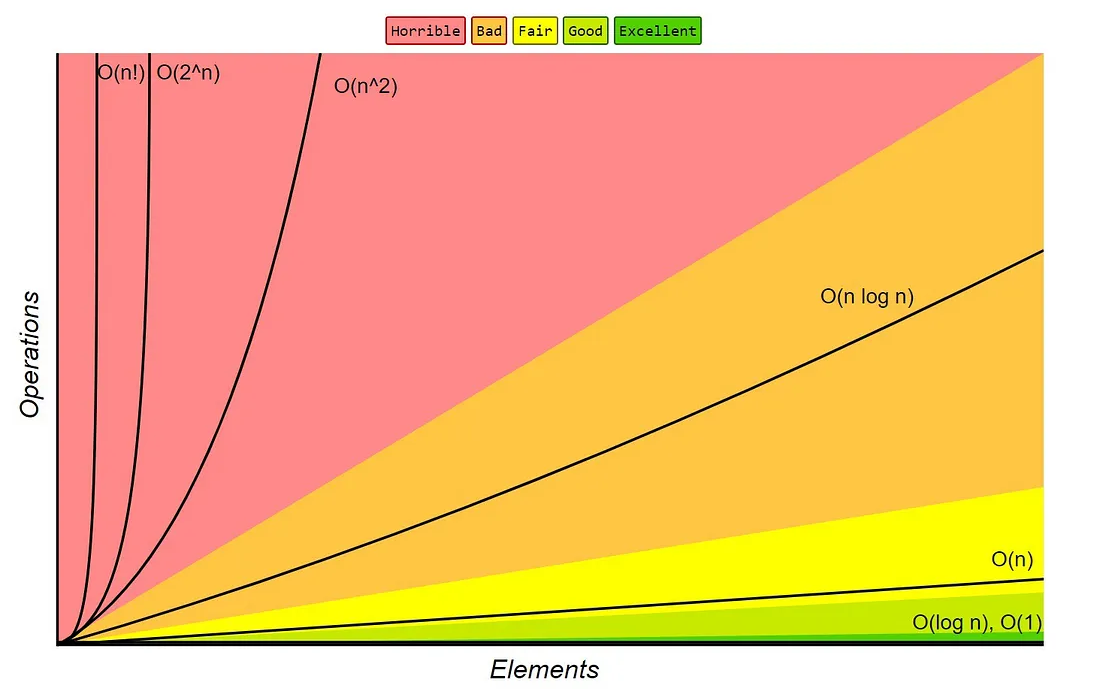
\includegraphics[width=0.6\textwidth]{./assets/images/Asymptotic Notations.png}
  \caption{Asymptotic Notation}
\end{figure}

\subsection{Big-O Notation}

The \textbf{\textit{big-O notation}} is used to describe the upper bound
on the growth rate of an algorithm as the input size approaches infinity.
It provides an upper limit on the worst-case time complexity of an algorithm.
The big-O notation is used to analyze the efficiency of an algorithm in terms
of the number of basic operations it performs.

\subsection{Omega Notation}

The \textbf{\textit{omega notation}} or \textbf{\textit{big-omega notation}}
is used to describe the lower bound on the growth rate of an algorithm as the
input size approaches infinity. It provides a lower limit on the best-case
time complexity of an algorithm. The omega notation is used to analyze the
efficiency of an algorithm in terms of the minimum number of basic operations
it performs.

\subsection{Theta Notation}

The \textbf{\textit{theta notation}} or \textbf{\textit{big-theta notation}}
is used to describe the tight bound on the growth rate of an algorithm as
the input size approaches infinity. It provides an upper and lower limit on
the time complexity of an algorithm. The theta notation is used to analyze
the efficiency of an algorithm in terms of the average number of basic
operations it performs.

\section{Summary}

In this chapter, we introduced the fundamental concepts of data structures
and algorithms. We discussed the importance of data structures and algorithms
in computer science and software engineering. We also covered some basic
terminologies related to data structures and algorithms, such as data, data
object, data type, abstract data type, and complexity of an algorithm. We
introduced the concept of asymptotic notations, such as big-O notation, omega
notation, and theta notation, and discussed the time complexity of algorithms
in terms of big-O notation. We covered common time complexity ranges from best
to worst performance, such as constant time complexity, logarithmic time
complexity, linear time complexity, linearithmic time complexity, quadratic
time complexity, exponential time complexity, and factorial time complexity.

%%%%%%%%%%%%%%%%%%%%%%%%%%%%%%%%%%%%
%%%%%~ NEW CHAPTER STARTS HERE %%%%%
%%%%%%%%%%%%%%%%%%%%%%%%%%%%%%%%%%%%
\chapter{Arrays and Linked Lists}

\section{Introduction}

\section{Arrays}

\subsection{Types of Arrays}

\subsubsection{One-dimensional Array}

\subsubsection{Multi-dimensional Array}

\subsection{Array Operations}

\subsubsection{Insertion}

\subsubsection{Deletion}

\subsubsection{Searching}

\subsection{Complexity Analysis of Arrays}

\section{Linked Lists}

\subsection{Types of Linked Lists}

\subsubsection{Singly Linked List}

\subsubsection{Doubly Linked List}

\subsubsection{Circular Linked List}

\subsection{Operations on Linked Lists}

\subsubsection{Insertion}

\subsubsection{Deletion}

\subsubsection{Searching}

\subsection{Complexity Analysis of Linked Lists}

\section{Comparison of Arrays and Linked Lists}

\section{Summary}

%%%%%%%%%%%%%%%%%%%%%%%%%%%%%%%%%%%%
%%%%%~ NEW CHAPTER STARTS HERE %%%%%
%%%%%%%%%%%%%%%%%%%%%%%%%%%%%%%%%%%%
\chapter{Stacks and Queues}

\section{Introduction}

\section{Stacks}

\subsection{Operations on Stacks}

\subsubsection{Push}

\subsubsection{Pop}

\subsubsection{Peek}

\subsubsection{isEmpty}

\subsubsection{isFull}

\subsection{Complexity Analysis of Stacks}

\subsection{Implementation of Stacks Using Arrays}

\subsection{Implementation of Stacks Using Linked Lists}

\section{Queues}

\subsection{Types of Queues}

\subsubsection{Linear Queue}

\subsubsection{Circular Queue}

\subsubsection{Priority Queue}

\subsubsection{Double-ended Queue (Deque)}

\subsection{Operations on Queues}

\subsubsection{Enqueue}

\subsubsection{Dequeue}

\subsubsection{Front}

\subsubsection{Rear}

\subsection{Complexity Analysis of Queues}

\subsection{Implementation of Queues Using Arrays}

\subsection{Implementation of Queues Using Linked Lists}

\section{Comparison of Stacks and Queues}

\section{Summary}

%%%%%%%%%%%%%%%%%%%%%%%%%%%%%%%%%%%%
%%%%%~ NEW CHAPTER STARTS HERE %%%%%
%%%%%%%%%%%%%%%%%%%%%%%%%%%%%%%%%%%%
\chapter{Trees}

\section{Introduction}

\section{Properties of Trees}

\subsection{Root Node}

\subsection{Parent Node}

\subsection{Child Node}

\subsection{Leaf Node}

\subsection{Ancestors}

\subsection{Siblings}

\subsection{Descendants}

\subsection{Height of a Tree}

\subsection{Depth of a Node}

\subsection{Degree of a Node}

\subsection{Level of a Node}

\subsection{Subtree}

\section{Types of Trees}

\subsection{Binary Tree}

\subsubsection{Types of Binary Trees}

\paragraph{Left-skewed Binary Tree}

\paragraph{Right-skewed Binary Tree}

\paragraph{Complete Binary Tree}

\subsection{Ternary Tree}

\subsection{N-ary Tree}

\subsection{Binary Search Tree}

\subsection{AVL Tree}

\subsection{Red-Black Tree}

\section{Basic Operations on Trees}

\subsection{Creation of a Tree}

\subsection{Insertion}

\subsection{Deletion}

\subsection{Searching}

\subsection{Traversal}

\subsubsection{Preorder Traversal}

\subsubsection{Inorder Traversal}

\subsubsection{Postorder Traversal}

\subsubsection{Level-order Traversal}

\section{Complexity Analysis of Trees}

\section{Summary}

%%%%%%%%%%%%%%%%%%%%%%%%%%%%%%%%%%%%
%%%%%~ NEW CHAPTER STARTS HERE %%%%%
%%%%%%%%%%%%%%%%%%%%%%%%%%%%%%%%%%%%
\chapter{Graphs}

\section{Introduction}

\section{Properties of Graphs}

\subsection{Vertex}

\subsection{Edge}

\subsection{Degree of a Vertex}

\subsection{Path}

\section{Types of Graphs}

\subsection{Finite Graph}

\subsection{Infinite Graph}

\subsection{Trivial Graph}

\subsection{Simple Graph}

\subsection{Multi Graph}

\subsection{Null Graph}

\subsection{Complete Graph}

\subsection{Pseudo Graph}

\subsection{Regular Graph}

\subsection{Bipartite Graph}

\subsection{Labelled Graph}

\subsection{Weighted Graph}

\subsection{Directed Graph}

\subsection{Undirected Graph}

\subsection{Connected Graph}

\subsection{Disconnected Graph}

\subsection{Cyclic Graph}

\subsection{Acyclic Graph}

\subsection{Directed Acyclic Graph (DAG)}

\subsection{Digraph}

\subsection{Subgraph}

\section{Operations on Graphs}

\subsection{Creation of a Graph}

\subsection{Insertion}

\subsubsection{Insertion of a Vertex}

\subsubsection{Insertion of an Edge}

\subsection{Deletion}

\subsubsection{Deletion of a Vertex}

\subsubsection{Deletion of an Edge}

\subsection{Traversal}

\subsubsection{Depth First Search (DFS)}

\subsubsection{Breadth First Search (BFS)}

\subsection{Shortest Path}

\subsection{Minimum Spanning Tree}

\section{Complexity Analysis of Graphs}

\section{Summary}

%%%%%%%%%%%%%%%%%%%%%%%%%%%%%%%%%%%%
%%%%%~ NEW CHAPTER STARTS HERE %%%%%
%%%%%%%%%%%%%%%%%%%%%%%%%%%%%%%%%%%%
\chapter{Sorting and Searching}

\section{Introduction}

\section{Sorting}

\subsection{Types of Sorting Algorithms}

\subsubsection{Bubble Sort}

\subsubsection{Selection Sort}

\subsubsection{Insertion Sort}

\subsubsection{Merge Sort}

\subsubsection{Quick Sort}

\subsubsection{Heap Sort}

\subsubsection{Radix Sort}

\subsubsection{Counting Sort}

\subsubsection{Bucket Sort}

\subsection{Comparison of Sorting Algorithms}

\section{Searching}

\subsection{Types of Searching Algorithms}

\subsubsection{Linear Search}

\subsubsection{Binary Search}

\subsubsection{Jump Search}

\subsubsection{Interpolation Search}

\subsubsection{Exponential Search}

\subsubsection{Fibonacci Search}

\subsubsection{Ternary Search}

\subsection{Comparison of Searching Algorithms}

\section{Summary}

%%%%%%%%%%%%%%%%%%%%%%%%%%%%%%%%%%%%
%%%%%~ NEW CHAPTER STARTS HERE %%%%%
%%%%%%%%%%%%%%%%%%%%%%%%%%%%%%%%%%%%
\chapter{Hashing}

\section{Introduction}

\section{Hash Table}

\section{Hash Function}

\section{Collision Resolution Techniques}

\subsection{Separate Chaining}

\subsection{Open Addressing}

\subsubsection{Linear Probing}

\subsubsection{Quadratic Probing}

\subsubsection{Double Hashing}

\section{Complexity Analysis of Hashing}

\section{Summary}

%%%%%%%%%%%%%%%%%%%%%%%%%%%%%%%%%%%%
%%%%%~ NEW CHAPTER STARTS HERE %%%%%
%%%%%%%%%%%%%%%%%%%%%%%%%%%%%%%%%%%%
\chapter{Advanced Data Structures and Algorithms}

\section{Introduction}

\section{Advanced Data Structures}

\subsection{Segment Tree}

\subsection{Fenwick Tree}

\subsection{Suffix Tree}

\subsection{Suffix Array}

\subsection{Trie}

\subsection{Heap}

\subsection{Disjoint Set}

\subsection{Skip List}

\subsection{Splay Tree}

\subsection{Bloom Filter}

\subsection{KD Tree}

\subsection{Quad Tree}

\subsection{Octree}

\subsection{B-Tree}

\subsection{B+ Tree}

\subsection{R-Tree}

\subsection{X-Tree}

\subsection{Y-Tree}

\subsection{Z-Tree}

\section{Advanced Algorithms}

\subsection{Dynamic Programming}

\subsection{Greedy Algorithms}

\subsection{Backtracking}

\subsection{Divide and Conquer}

\subsection{Branch and Bound}

\subsection{Randomized Algorithms}

\subsection{Approximation Algorithms}

\subsection{String Matching Algorithms}

\subsection{Pattern Searching Algorithms}

\subsection{Cryptography Algorithms}

\subsection{Geometric Algorithms}

\subsection{Graph Algorithms}

\subsection{Network Flow Algorithms}

\subsection{Game Theory Algorithms}

\subsection{Quantum Algorithms}

\section{Summary}

%%%%%%%%%%%%%%%%%%%%%%%%%%%%%%%%%%%%
%%%%%~ NEW CHAPTER STARTS HERE %%%%%
%%%%%%%%%%%%%%%%%%%%%%%%%%%%%%%%%%%%
\chapter{Applications of Data Structures and Algorithms}

\section{Applications in Computer Science}

\subsection{Operating Systems}

\subsection{Database Management Systems}

\subsection{Compiler Design}

\subsection{Networking}

\subsection{Artificial Intelligence}

\subsection{Machine Learning}

\subsection{Computer Graphics}

\subsection{Computer Vision}

\subsection{Robotics}

\subsection{Web Development}

\subsection{Mobile Development}

\subsection{Game Development}

\subsection{Cybersecurity}

\subsection{Quantum Computing}

\section{Applications in Real Life}

\subsection{Social Media}

\subsection{E-commerce}

\subsection{Healthcare}

\subsection{Finance}

\subsection{Transportation}

\subsection{Education}

\subsection{Agriculture}

\subsection{Manufacturing}

\subsection{Entertainment}

\subsection{Sports}

\subsection{Travel}

\subsection{Telecommunications}

\subsection{Energy}

\subsection{Environment}

\subsection{Politics}

\subsection{Military}

\section{Summary}

\chapter{References}

\begin{enumerate}[label={\textbf{\Alph*.}}]
  \item \textbf{Books}
    \begin{itemize}
      \item Vishwas R. (2023). Data Structure Handbook. Dr. Vishwas Raval. ISBN: 978-9359063591
      \item Cormen, T. H., Leiserson, C. E., Rivest, R. L., \& Stein, C. (2022). Introduction to algorithms. MIT press. ISBN: 978-0262046305
      \item Erickson, J. (2019). Algorithms. ISBN: 978-1792644832
    \end{itemize}
  \item \textbf{Other Sources}
    \begin{itemize}
      \item Tutorialspoint. (n.d.). Data Structures Basics. Data Structure Basics. \url{https://www.tutorialspoint.com/data_structures_algorithms/data_structures_basics.htm}
      \item Algorithm Archive · Arcane Algorithm Archive. (n.d.). \url{https://www.algorithm-archive.org/}
    \end{itemize}
\end{enumerate}

\end{document}
